\documentclass{beamer}

\useoutertheme[subsection=false]{miniframes}
\usecolortheme{beaver}
\setbeamertemplate{navigation symbols}{}
\setbeamertemplate{footline}{}
\usepackage{graphicx}
\usepackage{url}
\usepackage{datetime}

\usepackage{tikz-cd}

\newcommand {\framedgraphic}[3] {
  \begin{frame}{#1}
    \vspace{-0.5cm}
    \begin{center}
      \includegraphics[width=0.9\textwidth,keepaspectratio]{#2}
    \end{center}
    \vspace{-1cm}
    \begin{center}
      #3
    \end{center}
  \end{frame}
}
\newcommand{\lectureDate}{\formatdate{11}{10}{2018}}

\setbeamertemplate{caption}{\raggedright\insertcaption\par}
\title{MATH211: Linear Methods I}
\author{Matthew Burke}
\date{\lectureDate}
\begin{document}

\frame{\titlepage}

\begin{frame}{Lecture on \lectureDate}
  \tableofcontents
\end{frame}

\section*{Last time}
\label{sec:Last-time}

\begin{frame}{Last time}
  \begin{itemize}
  \item Eulidean space\vfill
  \item Addition scalar multiplication etc..\vfill
  \item Lines and planes in $\mathbb R^2$ and $\mathbb R^3$
  \end{itemize}
\end{frame}

\section{Lines and planes}

\begin{frame}
  \begin{beamercolorbox}[sep=12pt,center]{part title}
    \usebeamerfont{section title}\insertsection\par
  \end{beamercolorbox}
\end{frame}


\begin{frame}{Two dimensions}
  \begin{definition}
    A \emph{parametric (vector) equation} describing a line in $\mathbb R^2$ is a vector equation of the form
    \begin{equation*}
      \vec{x} = \vec{c}+s\vec{d}
    \end{equation*}
    for $\vec{x}$, $\vec{c}$ and $\vec{d}$ in $\mathbb R^2$ and $s$ in $\mathbb R$.
  \end{definition}\vfill
  \begin{definition}
    A \emph{parametric (vector) equation} describing a line in $\mathbb R^3$ is a vector equation of the form
    \begin{equation*}
      \vec{x} = \vec{c}+s\vec{d}
    \end{equation*}
    for $\vec{x}$, $\vec{c}$ and $\vec{d}$ in $\mathbb R^3$ and $s$ in $\mathbb R$.
  \end{definition}
\end{frame}

\begin{frame}{Parametric forms of 3D lines and planes}
  \begin{definition}
    A \emph{parametric (vector) equation} describing a plane in $\mathbb R^3$ is a vector equation of the form
    \begin{equation*}
      \vec{x} = \vec{c}+s\vec{d}+t\vec{e}
    \end{equation*}
    for $\vec{x}$, $\vec{c}$, $\vec{d}$ and $\vec{e}$ in $\mathbb R^3$ and $s$, $t$ in $\mathbb R$.
  \end{definition}\vfill
  \begin{definition}[Symmetric form of equation for line]
    \begin{equation*}
      \frac{x_1+b_1}{a_1} = \frac{x_2+b_2}{a_2} =\frac{x_3+b_3}{a_3}
    \end{equation*}
    where $a_i\neq 0$.
  \end{definition}
\end{frame}

\begin{frame}[fragile]{Converting between various forms}
  \begin{equation*}
    \begin{tikzcd}
      {}&\text{System of equations} \arrow{ddr}{\text{Row reduction}} &{}\\
      {}&{}&{}\\
      \text{Symmetric form} \arrow{uur}{\text{Split and rearrange}} &{} & \text{Parametric form} \arrow{ll}{\text{Eliminate parameter}}
    \end{tikzcd}
  \end{equation*}
\end{frame}

\begin{frame}{Conversion example}
    \begin{example}
    Write down all three forms for the line
    \begin{equation*}
      \left[
	\begin{array}{c}
          x_1\\
          x_2\\
          x_3
	\end{array}
      \right] = \left[
	\begin{array}{c}
          1\\
          -1\\
          2
	\end{array}
      \right]+s \left[
	\begin{array}{c}
          2\\
          1\\
          3
	\end{array}
      \right]
    \end{equation*}
  \end{example}
\end{frame}

\begin{frame}{Example}
   \begin{example}
    Write down a parametric equation for the line passing through
    \begin{equation*}
      \left[
	\begin{array}{c}
          4\\
          -7\\
          1
	\end{array}
      \right]
    \end{equation*}
    and parallel to the line
    \begin{equation*}
      \left[
	\begin{array}{c}
          x_1\\
          x_2\\
          x_3
	\end{array}
      \right] = \left[
	\begin{array}{c}
          4\\
          -7\\
          1
	\end{array}
      \right]+t \left[
	\begin{array}{c}
          2\\
          -5\\
          3
	\end{array}
      \right]
    \end{equation*}
  \end{example}
\end{frame}

\begin{frame}{Example}
  \begin{example}
    Write down the equation for the plane passing through the following three points.
    \begin{equation*}
      \left[
	\begin{array}{c}
          1\\
          0\\
          1
	\end{array}
      \right], \left[
	\begin{array}{c}
          1\\
          2\\
          0
	\end{array}
      \right], \left[
	\begin{array}{c}
          0\\
          0\\
          3
	\end{array}
      \right]
    \end{equation*}
  \end{example}
  \begin{example}
    For the following two lines find the point of intersection.
    \begin{equation*}
      \left[
	\begin{array}{c}
          x_1\\
          x_2\\
          x_3
	\end{array}
      \right] = \left[
	\begin{array}{c}
          3\\
          1\\
          3
	\end{array}
      \right]+ t \left[
	\begin{array}{c}
          1\\
          -2\\
          3
	\end{array}
      \right]\text{ and }
      \left[
	\begin{array}{c}
          x_1\\
          x_2\\
          x_3
	\end{array}
      \right] = \left[
	\begin{array}{c}
          4\\
          6\\
          1
	\end{array}
      \right]+ t \left[
	\begin{array}{c}
          2\\
          3\\
          1
	\end{array}
      \right]
    \end{equation*}
  \end{example}
\end{frame}

\section{Scalar product}

\begin{frame}
  \begin{beamercolorbox}[sep=12pt,center]{part title}
    \usebeamerfont{section title}\insertsection\par
  \end{beamercolorbox}
\end{frame}

\begin{frame}{Length of a vector}
  \begin{definition}[Two dimensions]
    If $
      \left[
	\begin{array}{c}
          x_1\\
          x_2
	\end{array}
      \right]$
    then $\| \vec{x} \| = \sqrt{x_1^2+x_2^2}$
  \end{definition}
  \begin{definition}[Three dimensions]
    If $\vec{x}=
      \left[
	\begin{array}{c}
          x_1\\
          x_2\\
          x_3
	\end{array}
      \right]$
    then $\| \vec{x} \| = \sqrt{x_1^2+x_2^2+x_3^2}$
  \end{definition}
  \begin{definition}[n dimensions]
    If $\vec{x}=
      \left[
	\begin{array}{c}
          x_1\\
          x_2\\
          \vdots \\
          x_n
	\end{array}
      \right]$
    then $\| \vec{x} \| = \sqrt{x_1^2+x_2^2+\dots +x_n^2}$
  \end{definition}
\end{frame}

\begin{frame}{Distance between two points}
  \begin{definition}[Two dimensions]
    If $\vec{x} =
    \left[
      \begin{array}{c}
        x_1\\
        x_2
      \end{array}
    \right]$ and $\vec{y} =
    \left[
      \begin{array}{c}
        y_1\\
        y_2
      \end{array}
    \right]$
    then $$d(\vec{x}, \vec{y}) = d(0, \vec{y}-\vec{x}) = \sqrt{(x_1-y_1)^2+(x_2-y_2)^2}$$
  \end{definition}
 \begin{definition}[Three dimensions]
    If $\vec{x} =
    \left[
      \begin{array}{c}
        x_1\\
        x_2\\
        x_3
      \end{array}
    \right]$ and $\vec{y} =
    \left[
      \begin{array}{c}
        y_1\\
        y_2\\
        y_3
      \end{array}
    \right]$
    then $$d(\vec{x}, \vec{y}) = d(0, \vec{y}-\vec{x}) = \sqrt{(x_1-y_1)^2+(x_2-y_2)^2+(x_3-y_3)^2}$$
  \end{definition}   
\end{frame}

\begin{frame}{N dimensions and scalar multiplication}
  \begin{definition}[n dimensions]
    If $\vec{x} =
      \left[
	\begin{array}{c}
          x_1\\
          x_2\\
          \dots\\
          x_n
	\end{array}
      \right]$ and $\vec{y} =
      \left[
	\begin{array}{c}
          y_1\\
          y_2\\
          \vdots\\
          y_n
	\end{array}
      \right]$
      then $$d(\vec{x}, \vec{y}) = d(0, \vec{y}-\vec{x}) = \sqrt{(x_1-y_1)^2+(x_2-y_2)^2+\dots +(x_n-y_n)^2}$$
    \end{definition}
    \begin{lemma}[Scalar multiplication]
      If $\vec{v}$ is a non-zero vector and $a$ is a scalar then
      \begin{equation*}
        \|a\vec{v}\| = |a|\|\vec{v}\|
      \end{equation*}
    \end{lemma}
\end{frame}

\begin{frame}{Examples}
  \begin{definition}
    A \emph{unit vector} is a vector with length equal to $1$.
  \end{definition}
  \begin{example}
    The following vectors are unit vectors:-
    \begin{equation*}
      \left[
	\begin{array}{c}
          1\\
          0\\
          0
	\end{array}
      \right],
      \left[
	\begin{array}{c}
          0\\
          1\\
          0
	\end{array}
      \right],
      \left[
	\begin{array}{c}
          0\\
          0\\
          1
	\end{array}
      \right],
      \left[
	\begin{array}{c}
          \sqrt{\frac{1}{2}}\\
          0\\
          - \sqrt{\frac{1}{2}}
	\end{array}
      \right]
    \end{equation*}
  \end{example}
\end{frame}

\begin{frame}{Examples}
  \begin{example}
    Find the distance between
    \begin{equation*}
      \left[
	\begin{array}{c}
          1\\
          -1\\
          3
	\end{array}
      \right]\text{ and }
      \left[
	\begin{array}{c}
          3\\
          1\\
          0
	\end{array}
      \right]
    \end{equation*}
  \end{example}
  \begin{example}
    Find the length of
    \begin{equation*}
      \left[
	\begin{array}{c}
          -3\\
          4
	\end{array}
      \right]\text{ and }
      \left[
	\begin{array}{c}
          3\\
          -1\\
          -2
	\end{array}
      \right]
    \end{equation*}
  \end{example}
\end{frame}

\begin{frame}{Scalar/dot product}
  \begin{definition}
    If $\vec{x}$ and $\vec{y}$ are in $\mathbb R^n$ then
    \begin{align*}
      \vec{x}\cdot\vec{y} &= \sum_{k=1}^n x_ky_k\\
                          &= x_1y_1+x_2y_2+\dots +x_ny_n
    \end{align*}
  \end{definition}\vfill
  And so in fact
  \begin{equation*}
    \|\vec{x}\| = \sqrt{\vec{x}\cdot\vec{x}}
  \end{equation*}
\end{frame}

\begin{frame}{Properties of the scalar product}
  \begin{theorem}
    Let $\vec{u}, \vec{v}, \vec{w}$ be vectors in $\mathbb R^3$ 
    (or $\mathbb R^2$) and let $k\in \mathbb R$.
    \begin{enumerate}
    \item $\vec{u}\cdot\vec{v}$ is a real number
    \item $\vec{u}\cdot\vec{v}=\vec{v}\cdot\vec{u}$
    \item $\vec{u}\cdot\vec{0}=0$
    \item $\vec{u}\cdot\vec{u}=\left|\vec{u}\right|^2$
    \item $(k\vec{u})\cdot\vec{v}=
k(\vec{u}\cdot\vec{v})=
\vec{u}\cdot(k\vec{v})$
\item $\vec{u}\cdot(\vec{v} + \vec{w}) =
\vec{u}\cdot\vec{v} + \vec{u}\cdot\vec{w}$

$\vec{u}\cdot(\vec{v} - \vec{w}) =
\vec{u}\cdot\vec{v} - \vec{u}\cdot\vec{w}$
\end{enumerate}
\end{theorem}
\end{frame}

\begin{frame}{Scalar product in terms of angle}
  \begin{columns}
    \column{0.5\textwidth}
    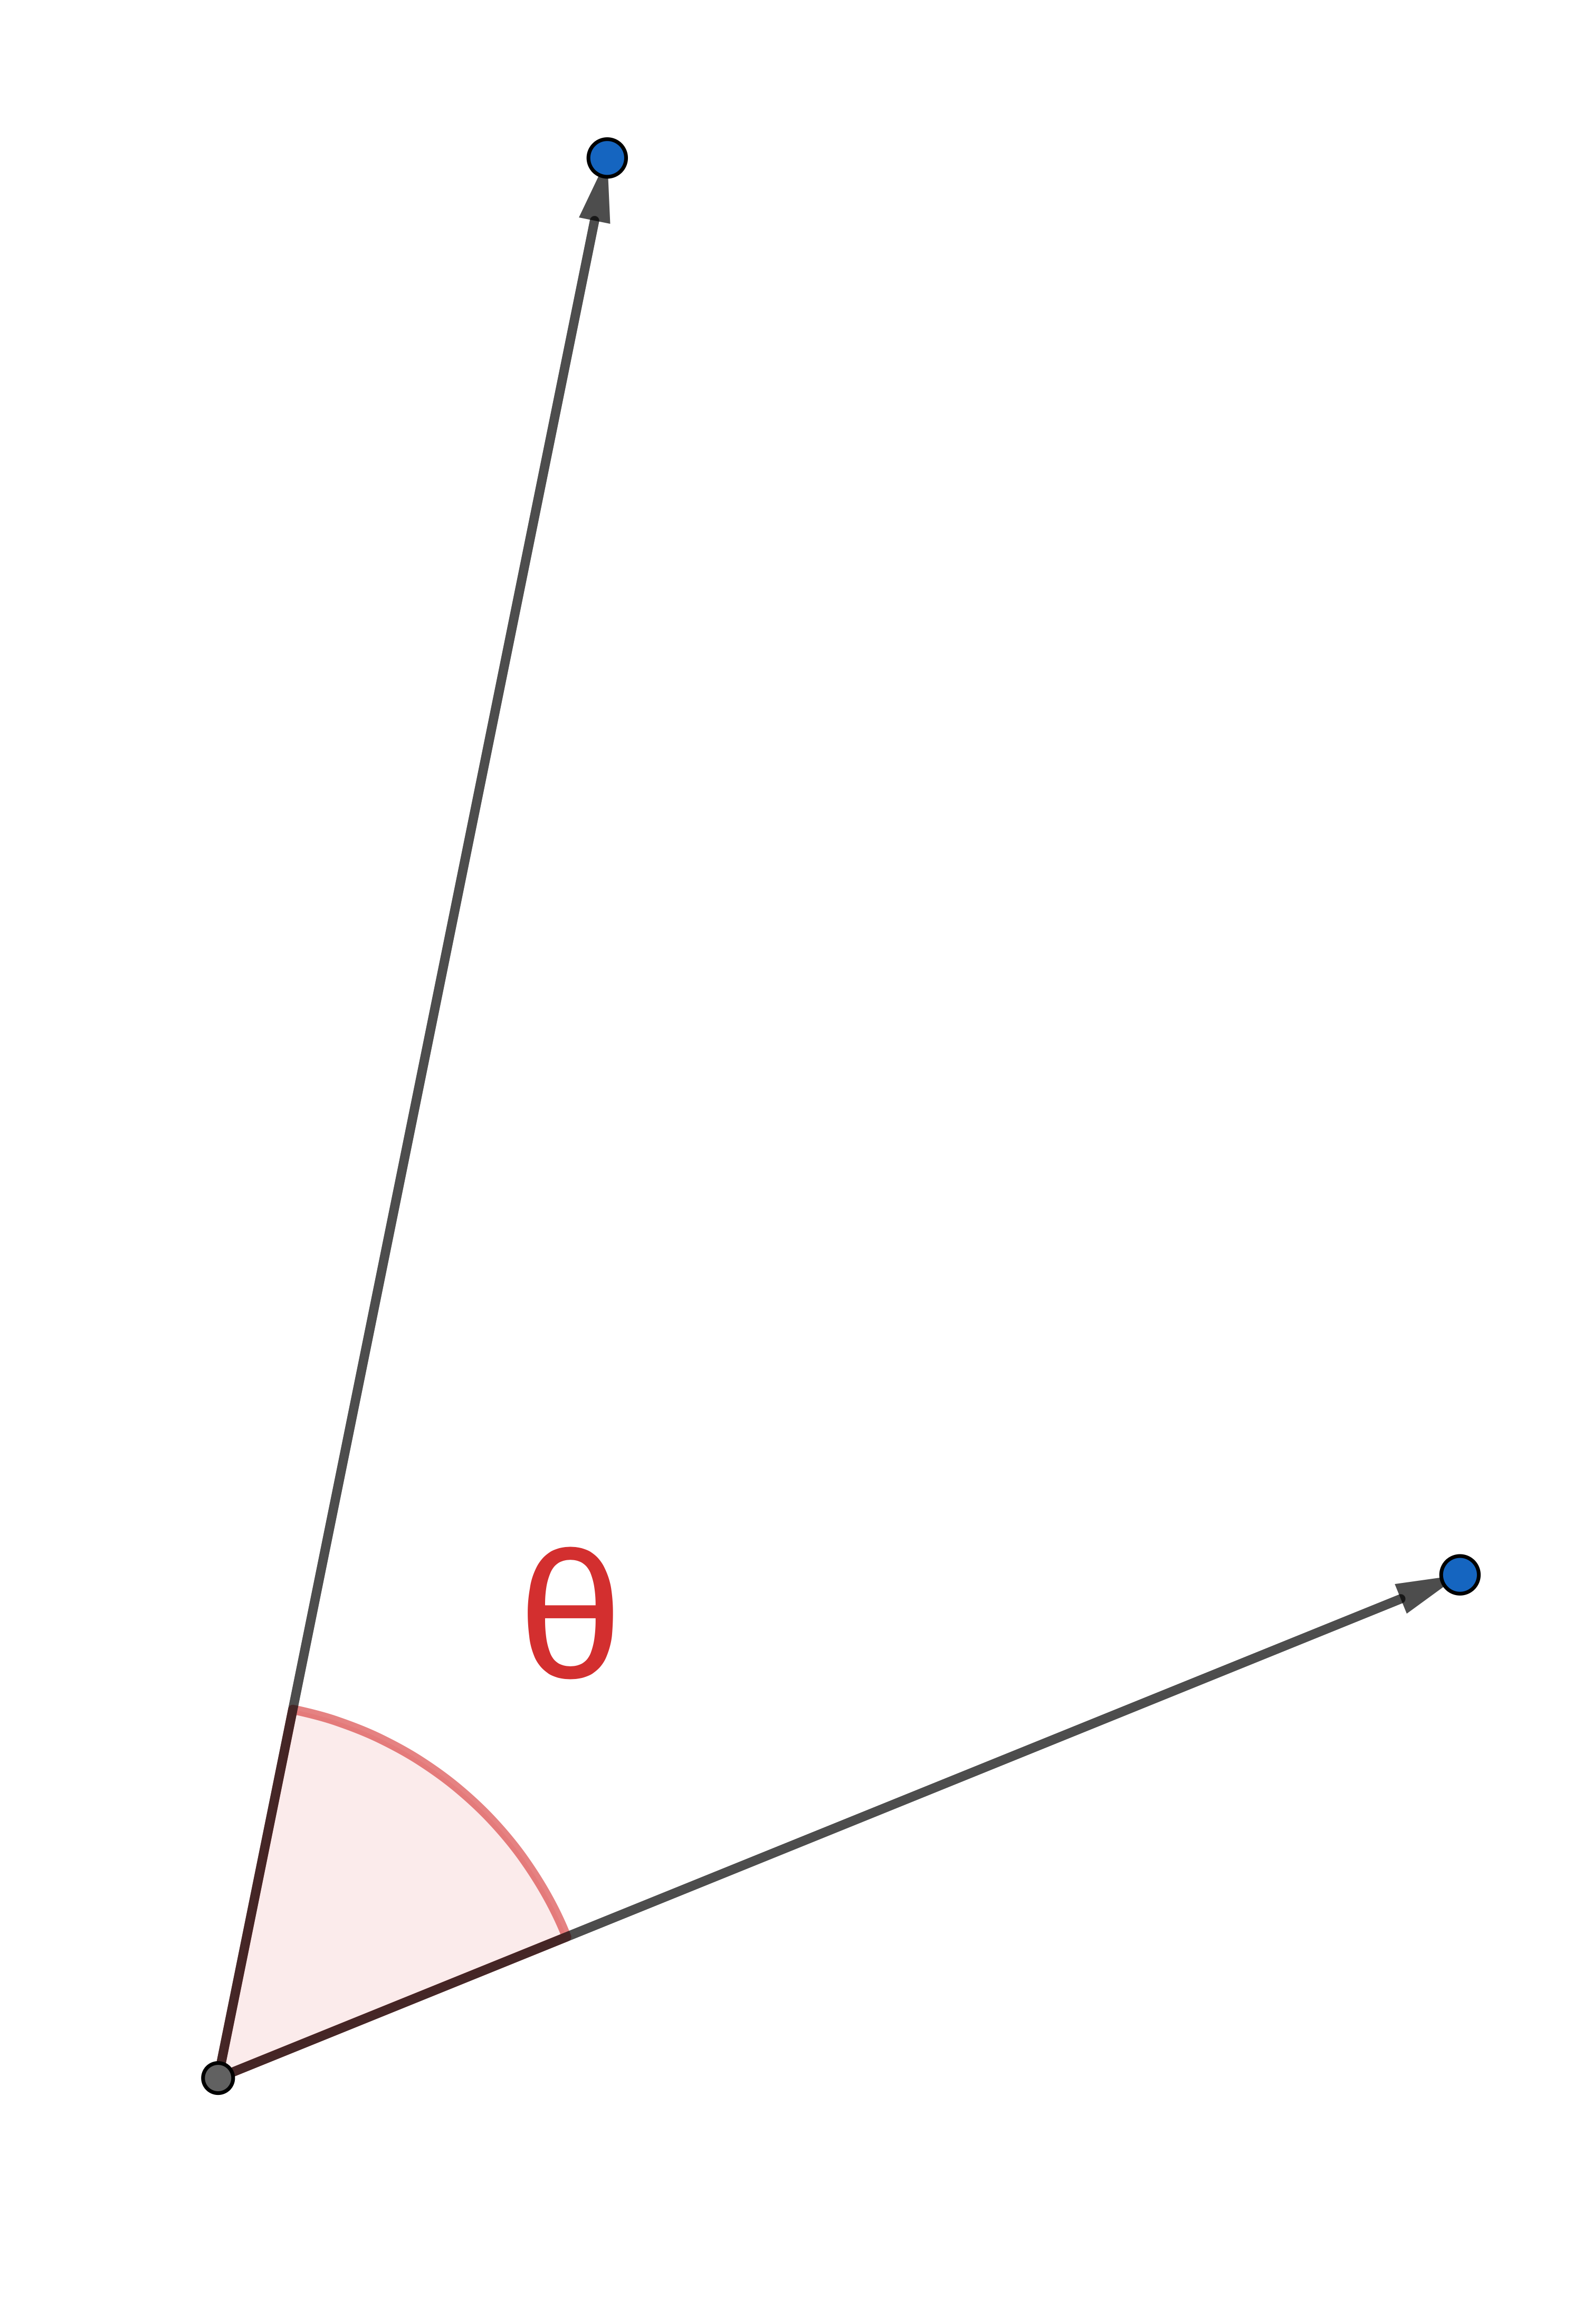
\includegraphics[scale=2]{angle.png}
    \column{0.5\textwidth}
    \begin{definition}[Scalar product in terms of angle]
      \begin{equation*}
        \vec{x}\cdot\vec{y} = |x||y|cos(\theta)
      \end{equation*}
    \end{definition}
  \end{columns}
\end{frame}

\begin{frame}{Examples}
  \begin{example}
    If \begin{equation*}
      u=\left[
	\begin{array}{c}
          1\\
          2\\
          0\\
          -1
	\end{array}
      \right]\text{ and }
      v = \left[
	\begin{array}{c}
          0\\
          1\\
          2\\
          3
	\end{array}
      \right]
    \end{equation*}
    then find $u\cdot v$.
  \end{example}
  \begin{example}
    Find the angle between
    \begin{equation*}
      \left[
	\begin{array}{c}
          1\\
          0\\
          -1
	\end{array}
      \right]\text{ and } \left[
	\begin{array}{c}
          0\\
          1\\
          -1
	\end{array}
      \right]
    \end{equation*}
  \end{example}
\end{frame}

\begin{frame}{Examples}
  \begin{example}
    Find the angle between
    \begin{equation*}
      \left[
	\begin{array}{c}
          7\\
          -1\\
          3
	\end{array}
      \right]\text{ and } \left[
	\begin{array}{c}
          1\\
          4\\
          -1
	\end{array}
      \right]
    \end{equation*}
  \end{example}
\end{frame}

\begin{frame}
  Questions?
\end{frame}

\section{Orthogonality}

\begin{frame}
  \begin{beamercolorbox}[sep=12pt,center]{part title}
    \usebeamerfont{section title}\insertsection\par
  \end{beamercolorbox}
\end{frame}

\begin{frame}{Orthogonality}
  \begin{definition}
    Two vectors $u$ and $v$ are \emph{orthogonal} iff
    \begin{equation*}
      u\cdot v = 0
    \end{equation*}
  \end{definition}\vfill
  Note that a zero vector is orthogonal to any other vector.
\end{frame}

\begin{frame}{Orthogonal complement}
  \begin{definition}[Slightly non-standard]
    If $v$ is a vector then the \emph{orthogonal complement $v^{\perp}$} of $v$ is the set of all vectors $u$ such that $u\cdot v = 0$.
  \end{definition}\vfill
  Therefore
  \begin{itemize}
  \item If $v\neq 0\in \mathbb R^1$ then $v^{\perp} = 0$.
  \item If $v\neq 0\in \mathbb R^2$ then $v^{\perp}$ is the line perpendicular to $v$.
  \item If $v\neq 0\in \mathbb R^2$ then $v^{\perp}$ is a plane.
  \end{itemize}\vfill
  In general if $v\neq 0 \in \mathbb R^n$ then $v^{\perp}$ is a $(n-1)$-dimensional subspace.
\end{frame}

\begin{frame}{Planes via normal vector}
  \begin{columns}
    \hspace{-1cm}
    \column{0.5\textwidth}
    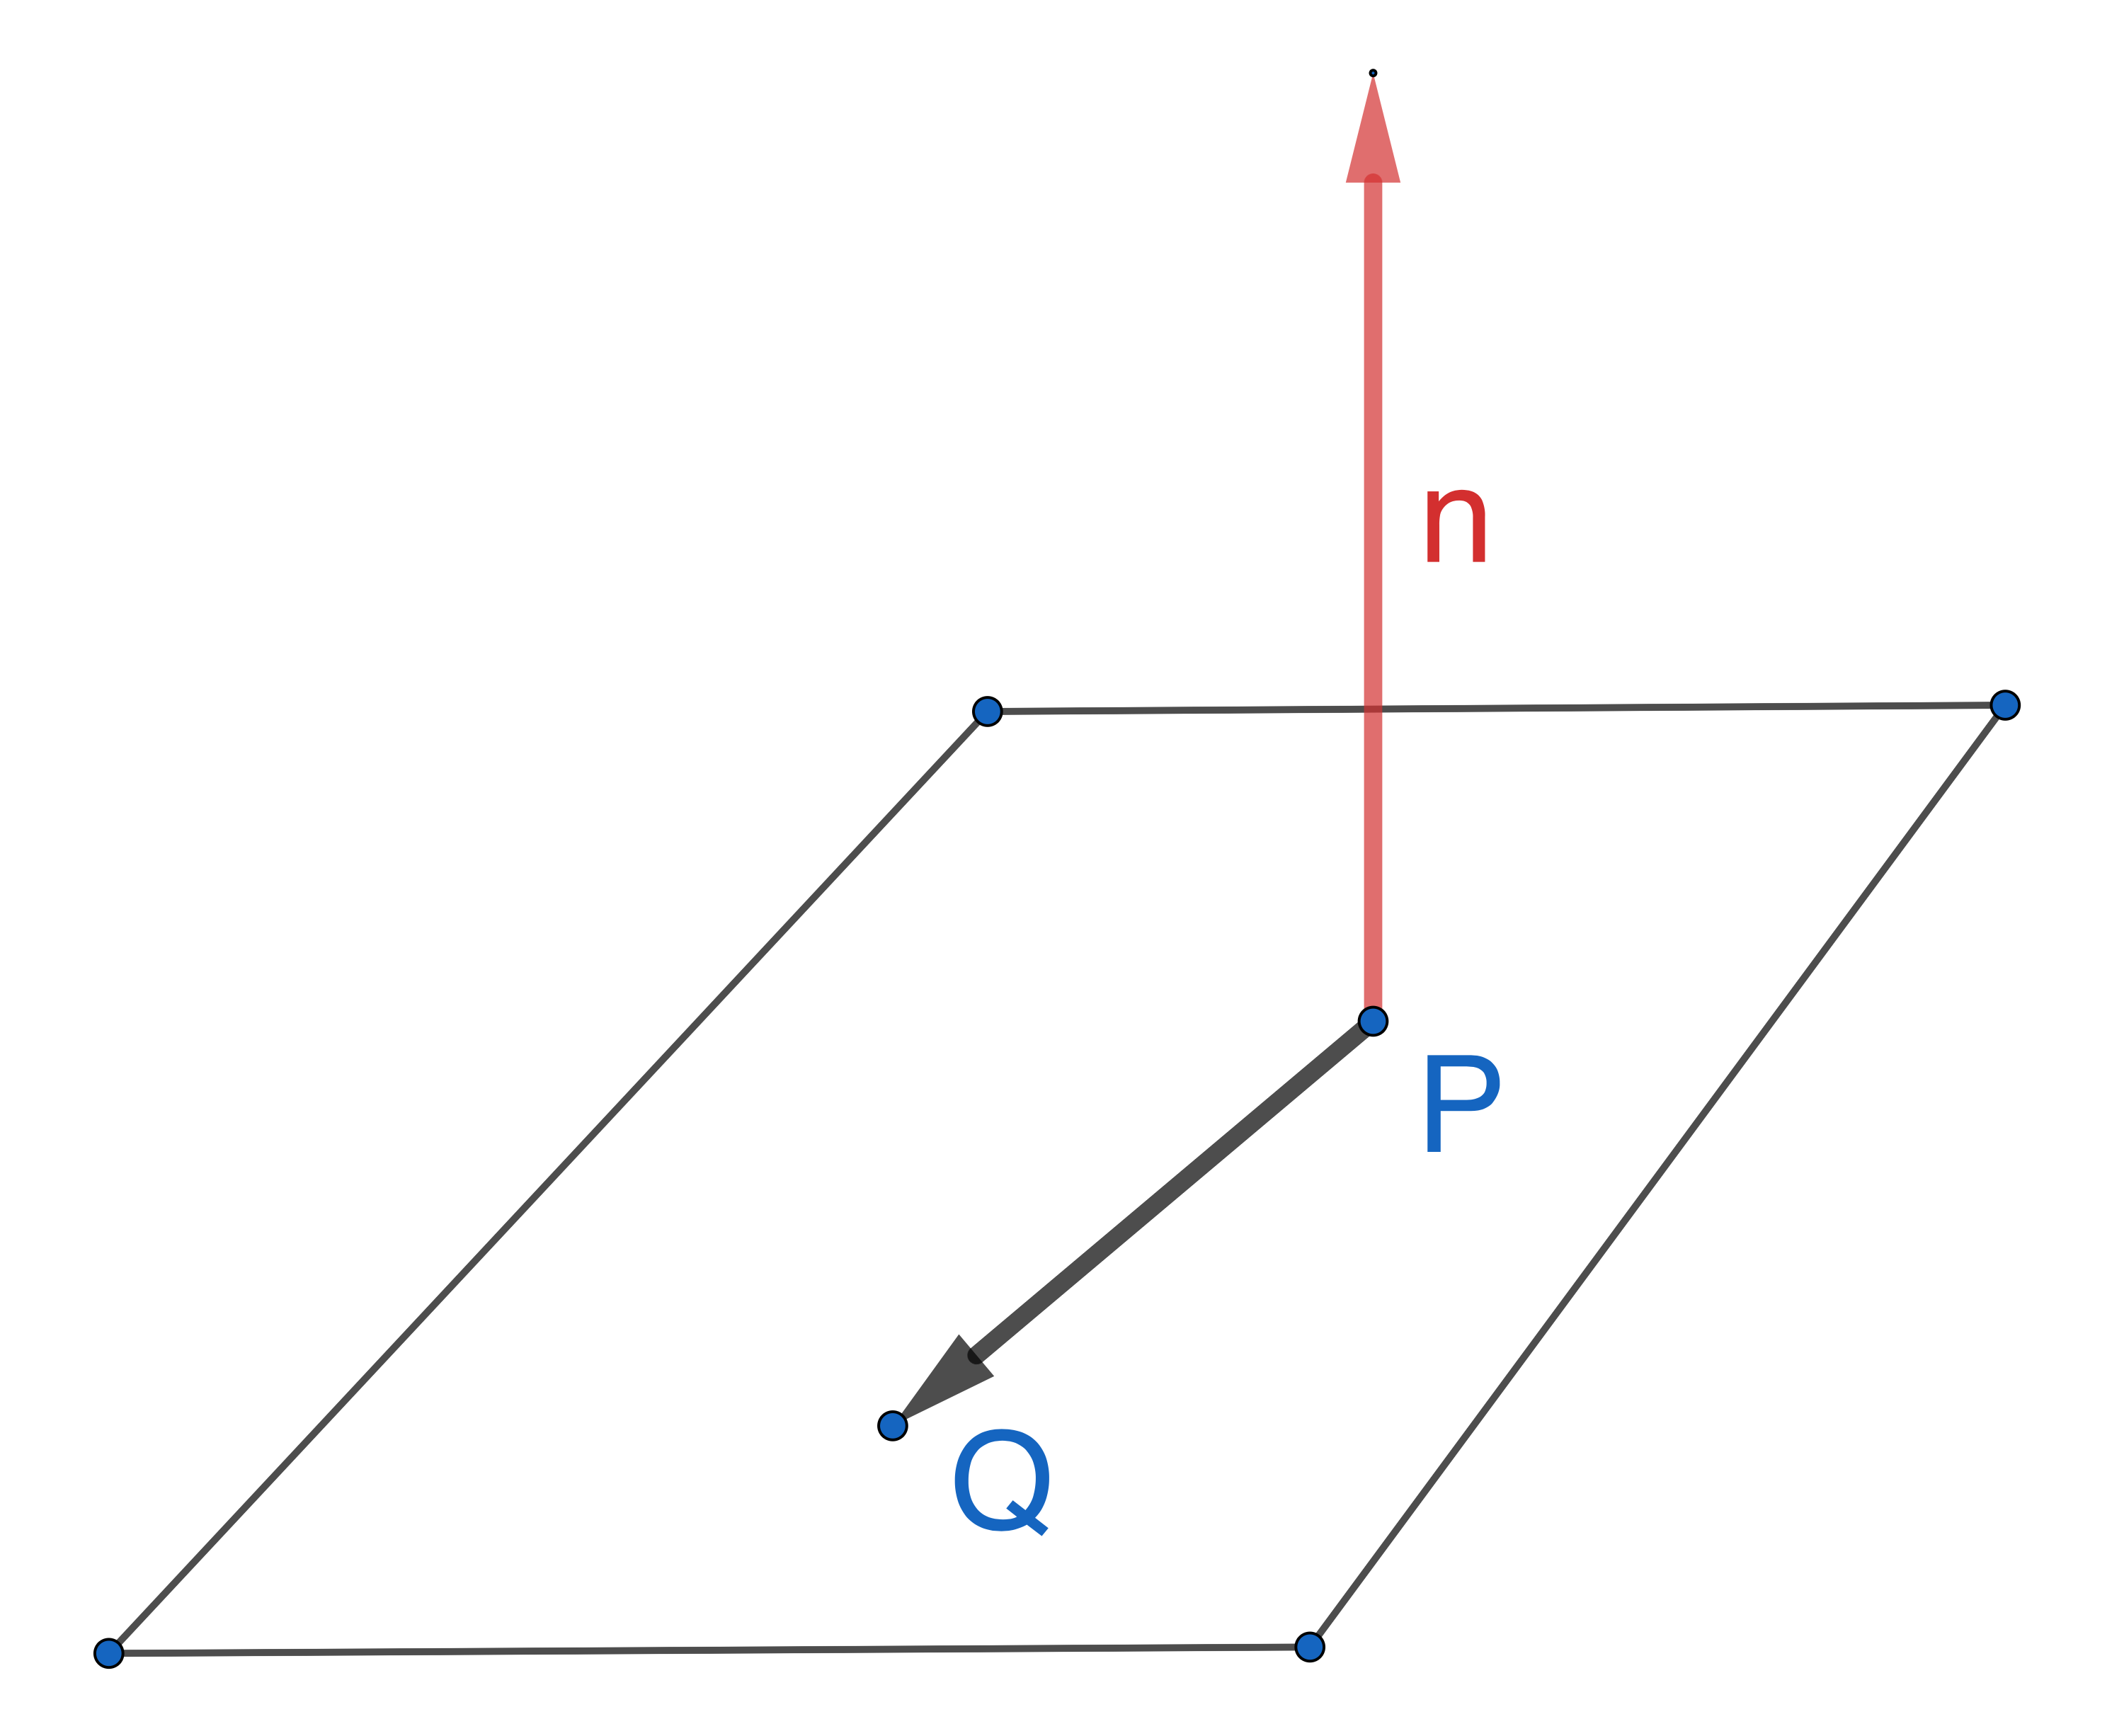
\includegraphics[scale=1]{normal-to-plane.png}
    \column{0.4\textwidth}
    \begin{itemize}
    \item Let $P$ be a point in the plane and $n$ a normal vector to the plane.
    \item For every point $Q$ in the plane the vector $\overrightarrow {PQ}$ is orthogonal to $n$.
    \item Therefore the solutions to
      \begin{equation*}
        n\cdot (x-P) = 0
      \end{equation*}
      form a plane.
    \end{itemize}
  \end{columns}
\end{frame}

\begin{frame}{Examples}
  \begin{example}
    Find all vectors orthogonal to both
    \begin{equation*}
      \left[
	\begin{array}{c}
          -1\\
          -3\\
          2
	\end{array}
      \right]\text{ and }
      \left[
	\begin{array}{c}
          0\\
          1\\
          1
	\end{array}
      \right]
    \end{equation*}
  \end{example}
  \begin{example}
    Are the following the vertices of a right angled triangle?
    \begin{equation*}
      \left[
	\begin{array}{c}
          4\\
          -7\\
          9
	\end{array}
      \right], \left[
	\begin{array}{c}
          6\\
          4\\
          4
	\end{array}
      \right], \left[
	\begin{array}{c}
          7\\
          10\\
          -6
	\end{array}
      \right]
    \end{equation*}
  \end{example}
\end{frame}

\begin{frame}{Example}
  \begin{example}
    Find an equation of the plane containing
    \begin{equation*}
      \left[
	\begin{array}{c}
          1\\
          -1\\
          0
	\end{array}
      \right]
    \end{equation*}
    orthogonal to
    \begin{equation*}
      \left[
	\begin{array}{c}
          -3\\
          5\\
          2
	\end{array}
      \right]
    \end{equation*}
  \end{example}
  \begin{example}
    A rhombus is a parallelogram with sides of equal length.
    Prove that the diagonals of a rhombus are perpendicular.
  \end{example}
\end{frame}

\begin{frame}
  Questions?
\end{frame}

\section{Projections}

\begin{frame}
  \begin{beamercolorbox}[sep=12pt,center]{part title}
    \usebeamerfont{section title}\insertsection\par
  \end{beamercolorbox}
\end{frame}

\begin{frame}{Projection onto a vector}
  \begin{columns}
    \column{0.5\textwidth}
    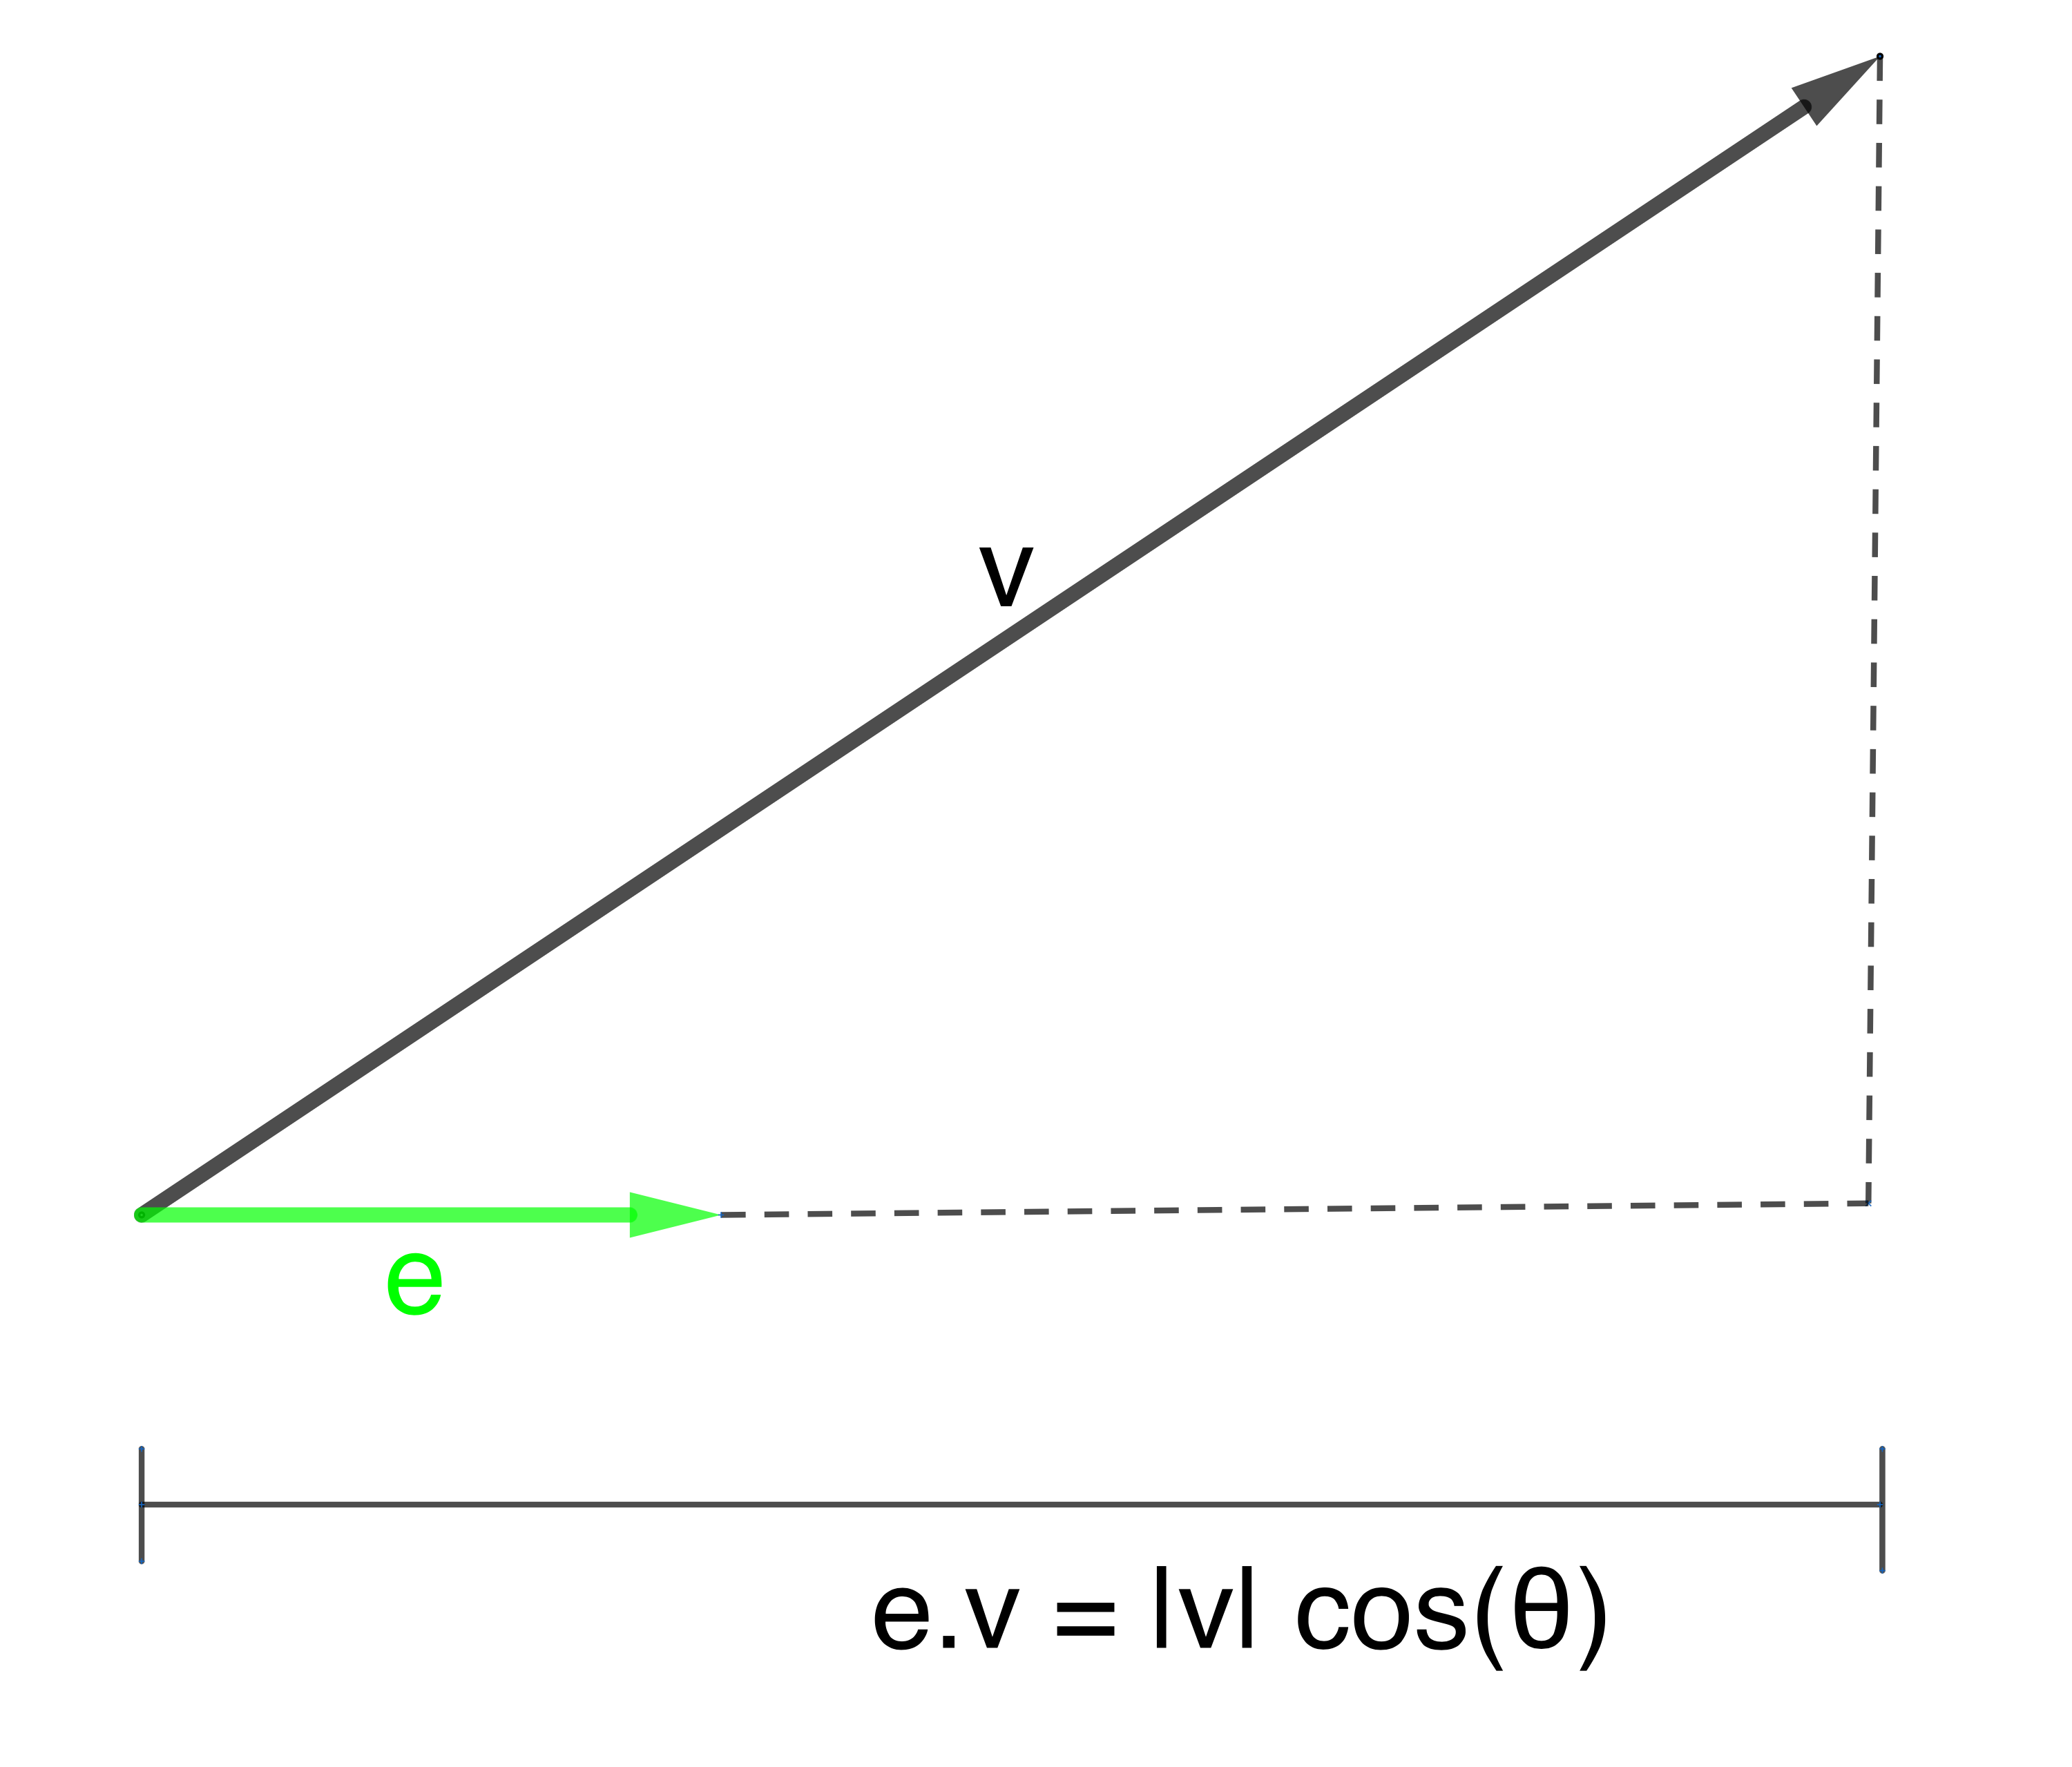
\includegraphics[scale=1.7]{projection-onto-unit.png}
    \column{0.4\textwidth}
    If $e$ is a unit vector then
    \begin{equation*}
      e\cdot v = |e||v|cos \theta = |v|cos \theta
    \end{equation*}
    and so $e\cdot v$ is the length of $v$ projected onto the line in direction $e$.
  \end{columns}
\end{frame}

\begin{frame}{Projection onto a vector}
  \begin{columns}
    \column{0.5\textwidth}
    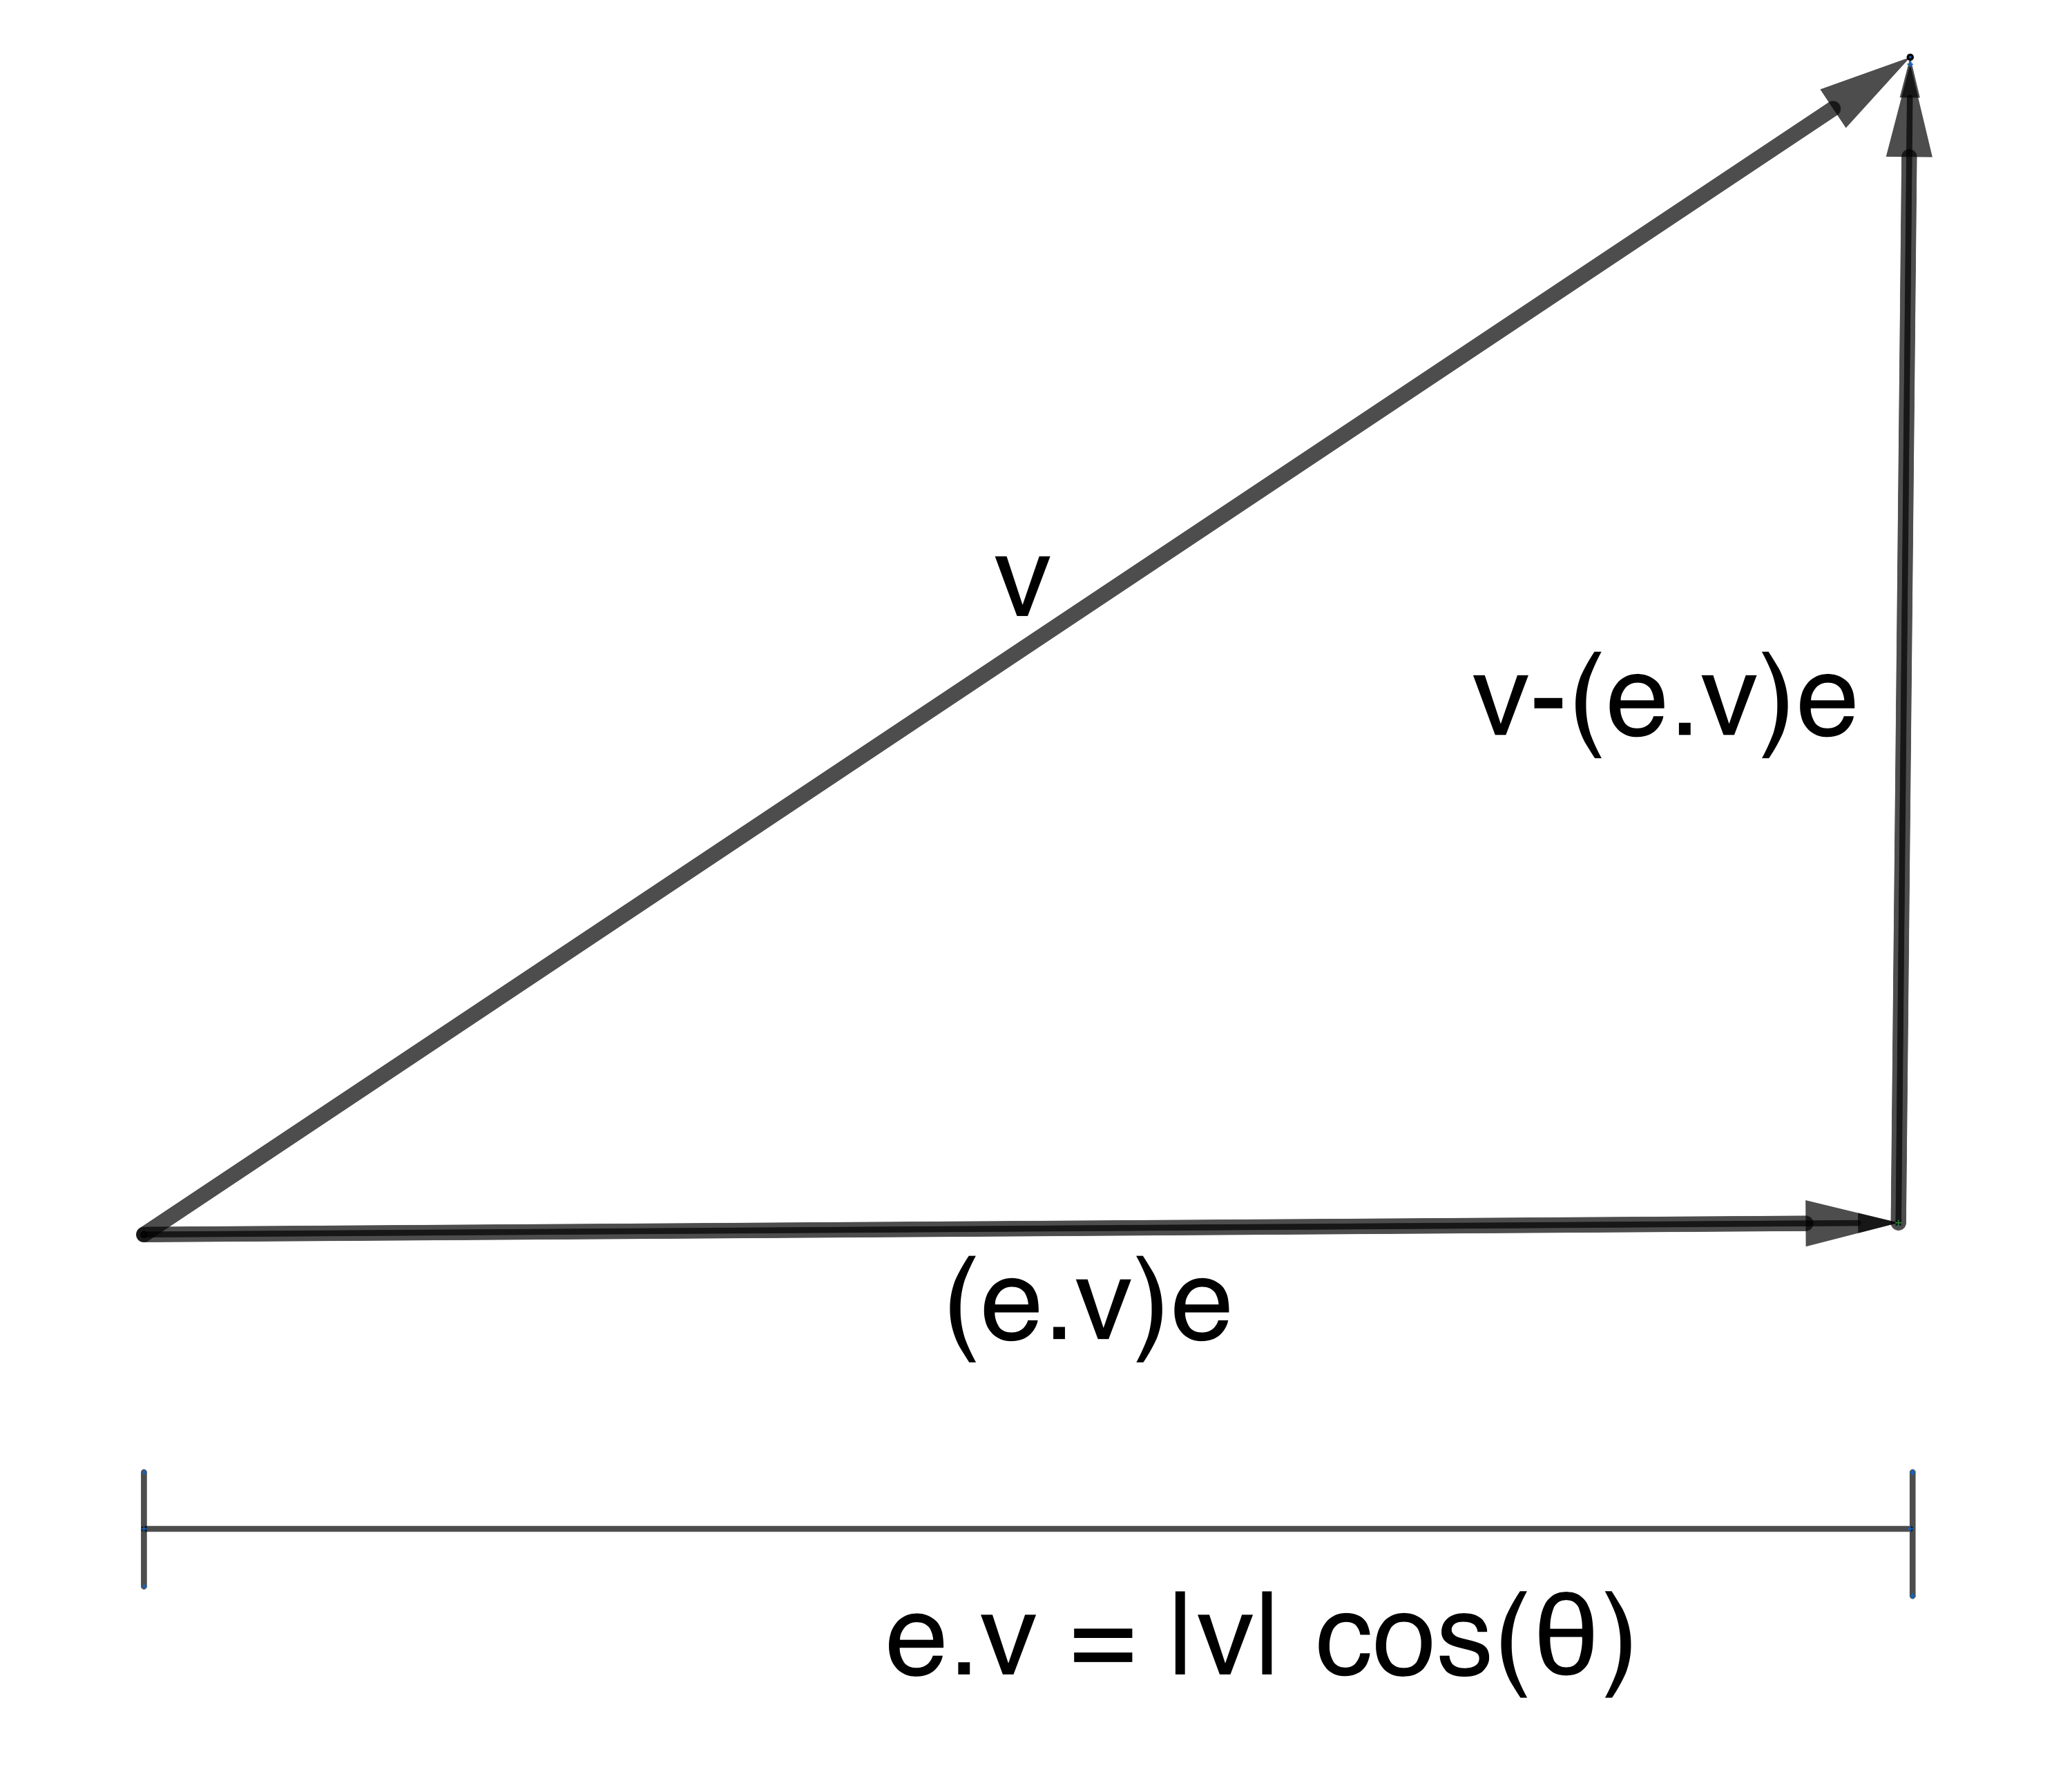
\includegraphics[scale=1.7]{decomposition-vector.png}
    \column{0.4\textwidth}
    Therefore we can write
    \begin{equation*}
      v = (e\cdot v)e + (v- e(e\cdot v))
    \end{equation*}
    where $(e\cdot v)e$ is parallel to $e$ and $(v- e(e\cdot v))$ is orthogonal to $e$.
  \end{columns}
\end{frame}

\begin{frame}{Examples}
  \begin{example}
    Let
    \begin{equation*}
      v = \left[
	\begin{array}{c}
          2\\
          -1\\
          0
	\end{array}
      \right]\text{ and }
      u = \left[
	\begin{array}{c}
          3\\
          1\\
          -1
	\end{array}
      \right]
    \end{equation*}
    Find vectors $v_0$ and $v_1$ such that $v = v_0 + v_1$, $v_0$ is orthogonal to $u$ and $v_1$ is parallel to $u$.
  \end{example}
\end{frame}

\begin{frame}{Example}
    \begin{example}
    If
    \begin{equation*}
      p= \left[
	\begin{array}{c}
          3\\
          2\\
          -1
	\end{array}
      \right]
    \end{equation*}
    find the closest point to $p$ on the following line:
    \begin{equation*}
      \left[
	\begin{array}{c}
          x_1\\
          x_2\\
          x_3
	\end{array}
      \right] = \left[
	\begin{array}{c}
          2\\
          1\\
          3
	\end{array}
      \right]+s \left[
	\begin{array}{c}
          3\\
          -1\\
          -2
	\end{array}
      \right]
    \end{equation*}
  \end{example}
\end{frame}

\begin{frame}{Example}
    \begin{example}
    Find the shortest distance from the point
    \begin{equation*}
      \left[
	\begin{array}{c}
          2\\
          3\\
          0
	\end{array}
      \right]
    \end{equation*}
    to the plane with equation $5x+y+z = -1$.
  \end{example}
\end{frame}

\begin{frame}
  Questions?
\end{frame}

\end{document}